\documentclass[aspectratio=43]{beamer}
\usepackage{ragged2e}

\usetheme{CSCS}


\newcommand{\SummerSchoolYear}{2016}
\newcommand{\SummerSchoolDate}{July 20 -- 21}
\newcommand{\SummerSchoolAuthor}{Maxime Martinasso}

\newcommand{\footlinetext}{Summer School \SummerSchoolYear{} -- MPI}

\author{\SummerSchoolAuthor, CSCS}
\title{Message Passing Interface (MPI)}
\subtitle{Summer School \SummerSchoolYear{}  -- Effective High Performance Computing}
\date{\SummerSchoolDate, \SummerSchoolYear}


% Select the image for the title page
\newcommand{\picturetitle}{cscs_images/image3.pdf}
%\newcommand{\picturetitle}{cscs_images/image5.pdf}
%\newcommand{\picturetitle}{cscs_images/image6.pdf}

\begin{document}

% TITLE SLIDE
\cscstitle

\begin{frame}{Why MPI?}
\begin{itemize}
    \item Distributed memory - use more nodes and cores
    \item Industry standards endorsed by many HPC actors
    \item Several implementations exist:
    \begin{itemize}
        \item Mpich, OpenMPI, IntelMPI, \textbf{CrayMPI},\ldots
    \end{itemize}
\end{itemize}
\end{frame}

\begin{frame}{Course prerequisites}
\begin{itemize}
    \item Basic C and/or Fortran knowledge
    \item Understand cluster architecture and tools
    \item Minimum understanding on Network metrics:
    \begin{itemize}
        \item Bandwidth: ratio of message size / time (GB/s)
        \item Latency: minimal time to send one bit ($\mu s$)
    \end{itemize}
    \item To think parallel !
\end{itemize}
\end{frame}

\begin{frame}{Course Objectives}
\begin{itemize}
\item The understanding of MPI’s essential concepts
\item Be able to use all basic features of MPI
\item Be able to write highly parallel HPC code
%\item Be able to use I/O and other system interfaces
\item Knowing what advanced features exist in MPI
\item The understanding of its pitfalls and tricky features
%\item This teaches you to program MPI for real
\end{itemize}
\end{frame}

\begin{frame}{Behind the course}
\begin{itemize}
    \item Full standard:\\\url{http://www.mpi-forum.org}
    \item Tutorials:\\\url{https://computing.llnl.gov/tutorials/mpi/}
    \item Books:
    \begin{itemize}
        \item Parallel Programming with MPI - Oct 96
        \item MPI: The Complete Reference - Sept 98
        \item Using MPI - 2nd Edition - Nov 99
    \end{itemize}
\end{itemize}
    {\textbf{A lot of references and tutorials on Internet!}}
\end{frame}

% TABLE OF CONTENT SLIDE
\cscstableofcontents[hideallsubsections]{General Course Structure}

\section{An introduction to MPI}
\cscstableofcontents[currentsection]{General Course Structure}

% CHAPTER SLIDE
\cscschapter{An introduction to MPI}

\subsection{MPI}
\begin{frame}{Message Passing Interface}
\justifying
\small
The Message Passing Interface (MPI) is a library specification for message-passing.
It is a standard API (Application Programming Interface) that can be used to create parallel applications.
The MPI standardization effort makes use of the most attractive features of a number of existing message passing systems, rather than selecting one of them and adopting it as the standard.\\
\begin{blue2block}{Key aspects}
\begin{itemize}
    \item A programming model NOT a programming language
    \item A set of functions to exchange messages between processes
    \item A standard that defines the behaviors of the MPI functions
    \item Bindings for C and Fortran
    \item[\color{cscsred}$\Rightarrow$] It is just a library!
\end{itemize}
\end{blue2block}
\end{frame}

\begin{frame}{History}
\begin{itemize}
\item Early 80's many communication libraries existed: PVM, LAM, P4,\ldots
\item 92: agreement to develop one generic library, MPI was born.
\item Many companies helped finance the standard: IBM, Cray,\ldots
\item 94: First version of the standard was released, MPI-1
\item 95: Mpich and Lam-MPI were the first implementations
\item 98: Second version of the standard was relapsed, MPI-2
\item 02: MPI implementations were MPI-2 compliant
\item 08: Third version of the standard was raised, MPI-3
\end{itemize}
\end{frame}

\begin{frame}{MPI Standard}
\begin{itemize}
\item This is a standard, not a user’s guide
\item It is designed to be unambiguous, not easy to follow.
\end{itemize}

\begin{blue2block}{MPI-1}
\begin{itemize}
\item Basic facilities: pt2pt, collective, topology, datatypes,\ldots
\item Most people use only a small fraction of it!
\end{itemize}
\end{blue2block}

\begin{blue2block}{MPI-2}
\begin{itemize}
\item Parallel I/O, dynamic process management, remote memory operations
\end{itemize}
\end{blue2block}

\begin{blue2block}{MPI-3}
\begin{itemize}
\item Fortran 2008 bindings, removes deprecated C++ bindings
\end{itemize}
\end{blue2block}

\end{frame}

\subsection{Distributed memory}
\begin{frame}{Message Passing Paradigm}
\begin{black1block}{}
\begin{itemize}
\item Resources are Local (differently from shared memory model)
\item Each process runs in a “isolated” environment. Interactions requires Messages Exchange
\item Messages can be: instructions, data, synchronization
\item Message Passing works also in a Shared Memory system
\item Time to exchange messages is much larger than accessing local memory
\end{itemize}
\end{black1block}
\begin{black1block}{}
Message Passing is a \textbf{COOPERATIVE} approach,\\based on \textbf{THREE} basic operations:
\begin{itemize}
    \item SEND (a message)
    \item RECEIVE (a message)
    \item SYNCHRONIZE
\end{itemize}
\end{black1block}
\end{frame}


\begin{frame}{Distributed memory}
\begin{blue1block}{Distributed Memory}
\begin{itemize}
\item A program is run as separate, independent processes
\item Independent processes do not share data
\item Processes interact only by message passing
\end{itemize}
\end{blue1block}
\begin{center}
\includegraphics<1>[scale=0.5]{01.MPI_Intro/cluster.pdf}
\includegraphics<2>[scale=0.5]{01.MPI_Intro/clustermpi.pdf}
\includegraphics<3>[scale=0.5]{01.MPI_Intro/clustermpicom.pdf}
\end{center}
\end{frame}

\begin{frame}{Send/Recv}

\begin{center}
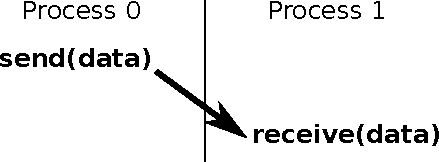
\includegraphics[scale=0.9]{01.MPI_Intro/sndrecv.pdf}
\end{center}

\begin{itemize}
\item description of data?
\item process identification?
\item when an operation is completed?
\end{itemize}
\end{frame}

\subsection{Using MPI in a program}
\begin{frame}{Using MPI in a program}
\begin{itemize}
\item Header files
\item Initialize and finalize MPI
\item Process identification
\item Simple communication model
\item Example of a simple source code
\end{itemize}
\end{frame}

\begin{frame}[fragile]{Header files}
All Subprogram that contains calls to MPI subroutine must include the MPI header file.\\
\begin{Pseudolisting}[]{}
#include <mpi.h>
\end{Pseudolisting}
\begin{Fortranlisting}[77]{}
include 'mpif.h'
\end{Fortranlisting}
\begin{Fortranlisting}[90]{}
USE MPI
\end{Fortranlisting}
The header file contains definitions of MPI constants, types and functions
\end{frame}


\begin{frame}[fragile]{MPI initialize and finalize}
\begin{itemize}
    \item Every MPI program starts by calling MPI\_Init:\\
\begin{Pseudolisting}[]{}
MPI_Init(argc, argv)
\end{Pseudolisting}
    \item Every MPI program ends by calling MPI\_Finalize\\
\begin{Pseudolisting}[]{}
MPI_Finalize()
\end{Pseudolisting}
\end{itemize}
\end{frame}

\begin{frame}{MPI communicators and ranks}
\begin{itemize}
    \item Every process has a MPI rank and belongs to an MPI communicator
    \item<2-> An MPI rank is an identification number
    \item<3-> An MPI communicator is a set of MPI rank
    \item<4-> Ranks are numbered locally to communicator
\end{itemize}
\begin{center}
\includegraphics<1>[scale=0.5]{01.MPI_Intro/clustermpi.pdf}
\includegraphics<2>[scale=0.5]{01.MPI_Intro/clustermpirank.pdf}
\includegraphics<3>[scale=0.5]{01.MPI_Intro/clustermpiworld.pdf}
\includegraphics<4>[scale=0.5]{01.MPI_Intro/clustermpi2com.pdf}
\end{center}

\end{frame}

\begin{frame}[fragile]{Process identification}
\begin{itemize}
    \item How many processes are associated with a communicator?\\
\begin{Pseudolisting}[]{}
MPI_Comm_size(MPI_Comm comm, size)
\end{Pseudolisting}[]{}
    \item How to get the rank of a process?\\
\begin{Pseudolisting}[]{}
MPI_Comm_rank(MPI_Comm comm, rank)
\end{Pseudolisting}[]{}
\end{itemize}
\end{frame}

\begin{frame}[fragile]{Simple MPI communication model}

Process with rank 1 sends to process with rank 2
\begin{Pseudolisting}[]{}
Rank 1: MPI_Send(<send data buffer>, 2, MyCommunicator)
Rank 2: MPI_Recv(<recv data buffer>, 1, MyCommunicator)
\end{Pseudolisting}

\visible<2->{
\begin{black0block}{}
\begin{itemize}
    \item same communicator: MyCommunicator
    \item send and recv buffer should be compatible:
        \begin{itemize}
        \item receive buffer should be large enough
        \item data type should match
        \end{itemize}
\end{itemize}
\end{black0block}
}

\visible<3->{
\begin{black0block}{}
\begin{itemize}
    \item Rank 2 is prepare to receive data from Rank 1
        \begin{itemize}
            \item \lstinlinePseudo{MPI_Recv} is called in "the right order" (deadlock)
        \item Rank 2 knows the maximum bound on the buffer size
        \end{itemize}
    \item[\color{cscsred}$\Rightarrow$]\textbf{\color{cscsred}Parallel!}
\end{itemize}
\end{black0block}
}

\end{frame}

\begin{frame}[fragile]{Example of MPI source code}
\begin{Cpplisting}[]{}
#include<mpi.h>
int main(int argc, char *argv[])
    int data[64];
    int nranks, my_rank;

    MPI_Init(&argc, &argv);
    MPI_Comm_size(MPI_COMM_WORLD, &nranks);
    MPI_Comm_rank(MPI_COMM_WORLD, &my_rank);
    assert(nranks % 2 == 0);// if not?

    if (my_rank % 2 == 0) {
        MPI_Send(data, 64, MPI_INT, my_rank+1, 0, MPI_COMM_WORLD);
    } else {
        MPI_Recv(data, 64, MPI_INT, my_rank-1, 0, MPI_COMM_WORLD, MPI_STATUS_IGNORE);
    }
    MPI_Finalize();
}
\end{Cpplisting}
\end{frame}


\subsection{MPI implementation insight}
\begin{frame}{MPI implementation insight}
\begin{itemize}
    \item[\color{cscsred}$\Rightarrow$]\textbf{\color{cscsred}Implementation dependent!}
\end{itemize}

\begin{blue1block}{Launcher: mpirun/srun}
\begin{itemize}
    \item Starts all process on all computer nodes (ssh)
    \item Attributes rank numbers by setting argc and argv
    \item Applies specific options like process pinning
\end{itemize}
\end{blue1block}

\begin{blue1block}{Library functions}
\begin{itemize}
    \item Setup process (rank, size) from launcher (argc, argv)
    \item Setup underlying network library (TCP, RDMA, \ldots)
    \item Process event coming from the application
        \begin{itemize}
        \item send, receive, wait, test, cancel,\ldots
        \end{itemize}
\end{itemize}
\end{blue1block}

\end{frame}

\subsection{MPI features}
\begin{frame}{MPI features}
\begin{itemize}
    \item Different flavors of point-to-point communications
    \begin{itemize}
        \item Blocking, non-blocking, synchronous, \ldots
    \end{itemize}
    \item Collective operations among ranks
    \begin{itemize}
        \item Broadcast, scatter, gather, reduce, alltoall, \ldots
    \end{itemize}
    \item Topology for managing rank numbering
    \begin{itemize}
        \item Cartesian topology, graph topology, \ldots
    \end{itemize}
    \item User specific data type (like C structure)
    \item Parallel I/O
    \begin{itemize}
        \item read and write files in parallel
    \end{itemize}
\end{itemize}
\end{frame}

\subsection{Practicals}
\begin{frame}{Practicals}
    \begin{brown2block}{Exercises: 01.MPI\_Intro}
    \begin{enumerate}
    \item Hello World!
    \item Hello World! with rank number
    \end{enumerate}
    \end{brown2block}
    \begin{brown0block}{Reminder}
        \lstinlinePseudo{srun -n 2 ./my_application my_args}\\
        Starts with 2 MPI ranks.
    \end{brown0block}
\end{frame}

\section{Point-to-point communications}
\section{Collective communications}
\section{Topology}
\section{Datatypes}

% THANK YOU SLIDE
\cscsthankyou{Thank you for your attention.}

\end{document}
